

\section*{Wprowadzenie} \addcontentsline{toc}{part}{Wprowadzenie} Niniejsze {\em Przepisy Ogólne Federacji Regnum Christi} obejmują normy uzupełniające {\em Statuty Federacji Regnum Christi}, które zostały zatwierdzone przez Stolicę Apostolską 31 maja 2019 roku i weszły w życie z dniem 15 września, tego samego, 2019 roku.

Normy uzupełniające zawarte w niniejszych Przepisach obowiązują całą Federację. W szczególny sposób określają one terytorialną oraz lokalną strukturę organizacyjną Federacji i jej poszczególnych instancji. Poniższy tekst, po wprowadzeniu minimalnych poprawek redakcyjnych i po dodaniu przewidzianych uprzednio przepisów uzupełniających, przywraca do życia teksty, które w grudniu 2018 roku zostały zatwierdzone przez Zgromadzenie Ogólne i pierwotnie były częścią Statutów, jednakże za radą Kongregacji ds. Instytutów Życia Konsekrowanego i Stowarzyszeń Życia Apostolskiego przeszły w skład niniejszych przepisów uzupełniających Federacji. Pozostałe, bardziej specyficzne normy zostały ujęte w innych przepisach ({\em Przepisy wiernych stowarzyszonych, Przepisy administracyjne, Przepisy terytorialne}).

Kolegium Generalne w porozumieniu z Plenarium Generalnym przyjmuje niniejsze {\em Przepisy Ogólne Federacji Regnum Christi} na próbny okres {\em ad experimentum} do momentu zwołania pierwszej Konwencji Generalnej Federacji Regnum Christi.

Rzym, 16 września 2019 roku.
\begin{center}
	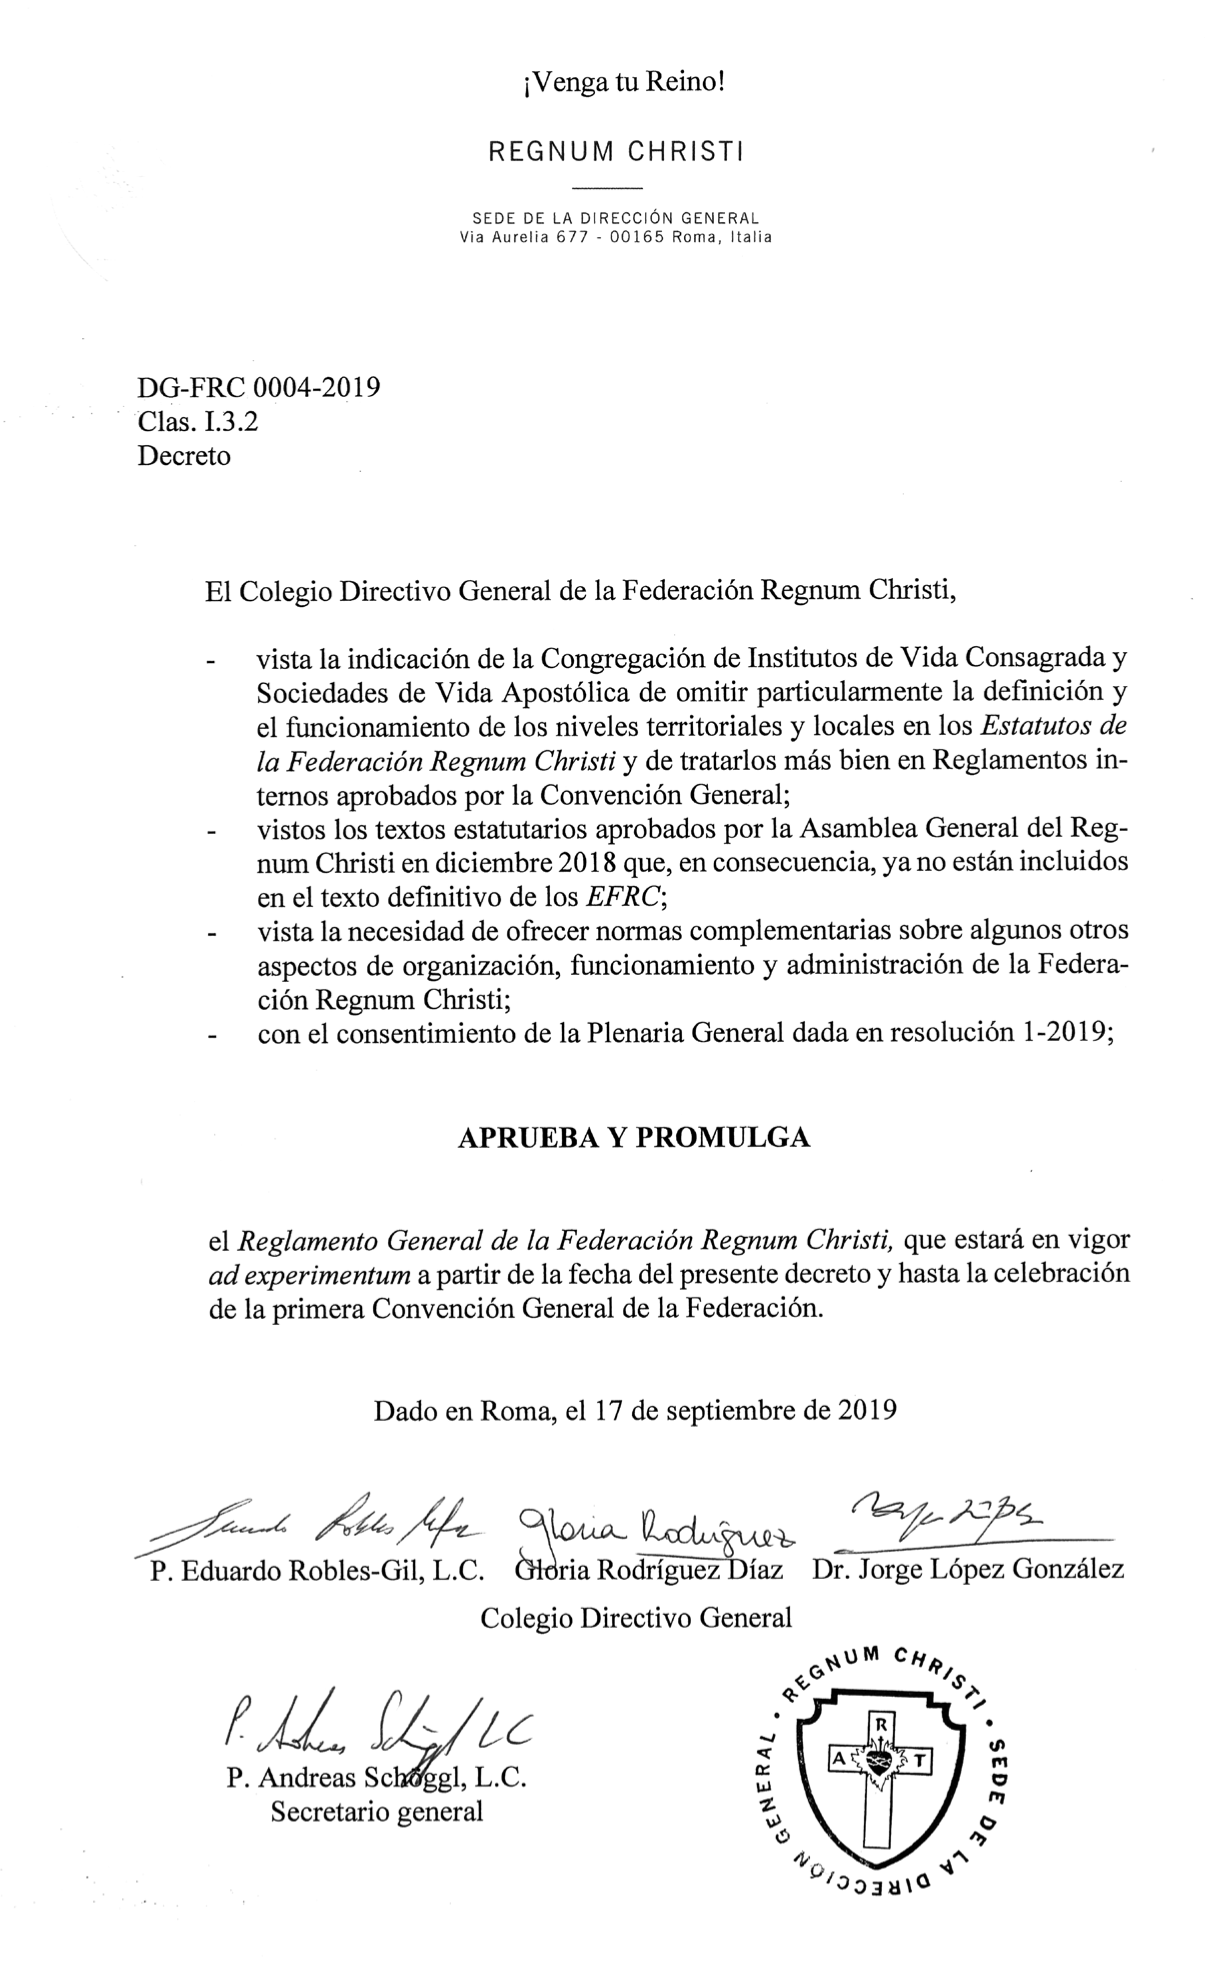
\includegraphics[height=
	\textheight]{dekret-przepisy-ogolne} 
\end{center}
\begin{framed}
	\setlength{
	\parskip}{.5em} 
	\begin{footnotesize}
		\begin{center}
			Przyjdź Królestwo Twoje!
			
			REGNUM CHRISTI
			
			{\tiny SIEDZIBA GENERALNEGO ZARZĄDU\\
			Via Aurelia 677, 00165 Rzym, Włochy} 
		\end{center}
		
		DG – FRC0004-2019\\
		Clas. I.3.2\\
		Dekret
		
		Kolegium Generalne Federacji Regnum Christi,
		\begin{itemize}
			
			\item na prośbę Kongregacji ds. Instytutów Życia Konsekrowanego i Stowarzyszeń Życia Apostolskiego, dotyczącą celowego pominięcia w tekście {\em Statutów Federacji Regnum Christi} punktu określającego funkcjonowanie poszczególnych terytorialnych i lokalnych szczebli Federacji, a następnie przeniesienia go do wewnętrznych przepisów zatwierdzonych przez Konwencję Generalną;
			
			\item po zapoznaniu się z punktami statutowymi zatwierdzonymi przez Generalne Zgromadzenie Regnum Christi w grudniu 2018 roku, lecz ostatecznie nie wchodzącymi w skład ostatniej wersji SFRC\footnote{\em Statutów Federacji Regnum Christi};
			
			\item uwzględniwszy potrzebę wprowadzenia przepisów uzupełniających niektóre kwestie dotyczące organizacji, funkcjonowania i zarządzania Federacji Regnum Christi;
			
			\item w porozumieniu z Plenarium Generalnym na mocy postanowienia 1-2019; 
		\end{itemize}
		\begin{center}
			\bf{}ZATWIERDZA I PRZYJMUJE
		\end{center}
		
		{\em Przepisy Ogólne Federacji Regnum Christi}, które wchodzą w życie na próbny okres {\em ad experimentum} wraz z datą niniejszego dekretu do momentu zwołania pierwszej Konwencji Generalnej Federacji.
		\begin{center}
			Podpisano w Rzymie, 17 września 2019 roku
			\begin{tabular}
				{ c c c } {\em podpis} & {\em podpis} & {\em podpis} \\
				o. Eduardo Robles-Gil, LC & Gloria Rodríguez Díaz & dr. Jorge López González \\
				\multicolumn{3}{c}{Kolegium Generalne} 
			\end{tabular}
			\begin{tabular}
				{ c c } {\em podpis} & \\
				o. Andreas Schöggl, LC & {\em pieczęć} \\
				Sekretarz Generalny & 
			\end{tabular}
		\end{center}
	\end{footnotesize}
\end{framed}

\setlength{
\parskip}{1em}

% Rozdział 1
\chapter{Przepisy ogólne w zakresie legislacji, organizacji i stanowienia władzy w Federacji}

\ssec{Przepisy terytorialne}

\lett{1} \S{}1. Przepisy terytorialne są zatwierdzane przez Kolegium Terytorialne w porozumieniu z Terytorialnym Plenarium. Zanim nastąpi ich ogłoszenie wymagana jest zgoda Kolegium Generalnego.

\S{}2. Kolegium Generalne, za zgodą Plenarium Generalnego, może zatwierdzać przepisy terytorialne zawierające wyjątki od prawa własnego w kwestii organizacji.

\ssec{Przepisy przejściowe regulujące skład pierwszej Konwencji Generalnej}

\lett{2} Opisane w punkcie 68 \S{}2 i \S{}4 Statutów Federacji Regnum Christi zasady wyboru osób na pierwszą Konwencję Generalną, określane są przez Kolegium Generalne w porozumieniu z Plenarium Generalnym.

\ssec{Konwencja terytorialna}

\lett{3} Przepisy regulujące skład, powołanie i formę Konwencji Terytorialnej wspomnianej w punkcie 70 {\em Statutów Federacji Regnum Christi}, ustalane są przez Kolegium Generalne po uprzedniej konsultacji z poszczególnymi terytoriami, zgodnie z {\em Przepisami Konwencji Generalnej} oraz punktem 40 {\em Przepisów wiernych stowarzyszonych w Federacji Regnum Christi}.

\ssec{Osobiste sprawowanie władzy przy wsparciu rady}

\lett{4} \S{}1. Dyrektor regionu, sekcji lub dzieła apostolskiego Federacji wspierany jest organem Rady, która pomaga mu w sprawowaniu władzy. Rada, na prośbę dyrektora, udziela mu swojej aprobaty lub opinii zgodnie z przepisami prawa własnego.

\S{}2. Dyrektor nie głosuje razem ze swoją Radą. Wyjątek stanowią sprawy, w których posiada on prawo głosu kolegialnego\footnote{Głos kolegialny jest wtedy, kiedy dyrektor generalny głosuje razem z swoimi doradcami.}.

\S{}3. O ile żadna z kompetentnych władz nie ustanowi inaczej, ważność głosowań Rady wymaga udziału co najmniej połowy członków\footnote{CIC, kanon 119, 3o; 127; 166.}.

\S{}4. Wprawdzie dyrektor nie ma żadnego obowiązku sugerowania się opinią Rady, nawet gdyby była ona jednogłośna, jednakże nie powinien bez powodu odstępować od wyrażonego przez niej stanowiska, zwłaszcza gdy jest ono zgodne i odpowiednio rozważone przed Bogiem\footnote{CIC, kanon 127 \S{}2, 2 o.}.

\S{}5. Członkowie poszczególnych rad zobowiązani są do szczerego wyrażania swej opinii, a także, gdy wymaga tego waga sprawy sprawy, do uważnego zachowywania tajemnicy, która może być kryterium wymaganym przez dyrektora\footnote{CIC, kanon 127 \S{}3.}.

\S{}6. Postanowienia paragrafów 4 i 5 niniejszego punktu mają zastosowanie w przypadku plenarium, które funkcjonuje jak Rada Kolegium Generalnego.

\ssec{Rejestr wiernych stowarzyszonych}

\lett{5} \S{}1. Każde terytorium zobowiązane jest do prowadzenia rejestru wiernych stowarzyszonych z uwzględnieniem aktualnych przepisów legislacji cywilnej odnośnie do ochrony danych osobowych oraz z uwzględnieniem wytycznych Kolegium Generalnego.

\S{}2. Wierni stowarzyszeni mogą wystosować prośbę o to, by ich imię nie pojawiało się w ogólnodostępnych rejestrach członków.

\S{}3. Jedynie wierni stowarzyszeni, którzy nie zastrzegli sobie prawa do upubliczniania swoich imion w ogólnodostępnych rejestrach członków mogą uczestniczyć w wyborach i obejmować stanowiska w Federacji.

\ssec{Archiwa Federacji}

\lett{6} Dyrekcja Generalna oraz Dyrekcje poszczególnych terytoriów Federacji zobowiązane są do prowadzenia archiwów. Odpowiada za nie sekretarz generalny lub sekretarz terytorialny. Chodzi o archiwa o charakterze eklezjalnym, podlegające prawu ogólnemu i prawu własnemu Federacji.

\filbreak\ssec{Ochrona nieletnich}

\lett{7} Kolegium Terytorialne we współpracy z instytucjami stowarzyszonymi odpowiada za wprowadzenie należytych przepisów oraz ich właściwe egzekwowanie w celu ochrony nieletnich, szczególnie w stosunku do osób biorących udział w aktywnościach Federacji. 

% Rozdział 2
\chapter{Nominacje}

\ssec{Organ odpowiedzialny za przyznawanie stanowisk w Federacji}

\lett{8} Organami, które mogą mianować innych na stanowiska są: Kolegium Generalne, Kolegium Terytorialne, dyrektor lokalny lub Kolegium zarządzające regionem, dyrektor sekcji oraz dyrektor dzieła lub programu apostolskiego.

\ssec{Nominacje członków instytucji stowarzyszonych}

\lett{9} \S{}1. Jeśli stanowisko w Federacji przyznawane jest jednemu z członków instytucji stowarzyszonych, zostaje on mianowany z ramienia Kolegium Generalnego lub Terytorialnego. Odbywa się to po uprzednim określeniu misji (apostolatu) przez odpowiedni organ instytucji stowarzyszonej i zgodnie z jej prawem własnym\footnote{SFRC, 52 \S{}1.}.

\S{}2. W przypadku nominacji na stanowiska wewnątrz regionów, sekcji, dzieł lub programów apostolatu, Kolegium Terytorialne powinno najpierw wysłuchać opinii stosownego dyrektora.

\ssec{Nominacje wiernych stowarzyszonych}

\lett{10} Mianowaniem wiernych stowarzyszonych zajmuje się kompetentny organ wskazany w punkcie 8. niniejszych {\em Przepisów} i po uprzedniej akceptacji stanowiska przez osobę zainteresowaną.

\ssec{Procedura}

\lett{11} \S{}1. Nominacje muszą odbywać się według określonej procedury, to znaczy ze wskazaniem stanowiska; okresu kadencji; zwierzchniego organu, przed którym będzie odpowiadać mianowana osoba; z zaznaczeniem pełnego etatu lub pół etatu pracy oraz ewentualnego wynagrodzenia.

\S{}2. Jeśli przepisy uzupełniające lub dekret nominacyjny nie stanowią inaczej o okresie trwania stanowiska, przyjmuje się ogólną praktykę trzech lat kadencji z możliwością jej przedłużenia.

\S{}3. Osoba odchodząca ze stanowiska, obejmująca stanowisko oraz organ zwierzchni odpowiadający za ciągłość tego stanowiska gwarantują uporządkowane i pełne przekazanie informacji.

\ssec{Sposób konsultacji}

\lett{12} Postępowanie w sprawie konsultacji poprzedzających nominację na stanowiska, wskazane w punkcie 60 {\em Statutów Federacji Regnum Christi}, musi być ściśle określone w przepisach terytorialnych Federacji.

\filbreak\ssec{Rezygnacja z funkcji przez członków instytucji stowarzyszonych}

\lett{13} \S{}1. Członek instytucji stowarzyszonej, który pragnie zrezygnować ze stanowiska pełnionego w Federacji powinien przedstawić swojemu dyrektorowi lub wyższemu przełożonemu pisemne podanie wyjaśniające powody swej decyzji. Powinien również o tym poinformować instancję odpowiedzialną za wykonywanie funkcji tego stanowiska.

\S{}2. Za przyjmowanie wniosków o dymisję swoich członków z funkcji w Federacji odpowiadają przełożeni i wyżsi dyrektorzy. Przed rozpatrzeniem wniosku o dymisję powinni oni zasięgnąć porady właściwego organu Kolegium Generalnego lub odpowiedniego dyrektora, w zależności od przypadku.

\ssec{Odsunięcie członków instytucji stowarzyszonych od funkcji w Federacji}

\lett{14} \S{}1. Członkowie instytucji stowarzyszonych mogą zostać odsunięci od funkcji na podstawie decyzji kierownictwa Federacji, która wystosowuje takie zalecenie do przełożonego lub odpowiedniego dyrektora stowarzyszonej instytucji albo na podstawie decyzji samego przełożonego lub właściwego dyrektora instytucji stowarzyszonej, po uprzednim przekazaniu takiej informacji do powiązanych instancji Federacji. W obu przypadkach nie jest wymagana zgoda drugiej strony, mimo tego należy postępować ostrożnie i dążyć do wzajemnego porozumienia.

\S{}2. W sytuacjach poważnych i pilnych (szkody na zdrowiu fizycznym i psychicznym, możliwego skandal lub upadłości apostolatu) odpowiedni przedstawiciel Federacji lub instytucji stowarzyszonych może niezwłocznie odsunąć daną osobę od pełnionej funkcji.

\filbreak\ssec{Rezygnacja lub odsunięcie wiernych stowarzyszonych}

\lett{15} \S{}1. Wierni stowarzyszeni, którzy dobrowolnie pragną zrezygnować z pełnionych w Federacji funkcji muszą przedstawić pisemną rezygnację organowi, który ich wcześniej powołał na stanowisko. 

\S{}2. Z wyjątkiem przypadków działania siły wyższej, zostaje wyznaczona taka data rozwiązania funkcji, która umożliwi właściwą procedurę przekazania obowiązków.

\S{}3. Za odsunięcie wiernych stowarzyszonych z ich funkcji odpowiada organ, który mianował ich na to stanowisko. Lokalni dyrektorzy, dyrektorzy sekcji, dzieł i programów apostolskich postępują w oparciu o opinię własnej Rady.

%
% Rozdział 3
\chapter{Przepisy uzupełniające dla Kolegium Generalnego oraz Plenarium Generalnego}

\ssec{Możliwość zwolnienia z przestrzegania danego przepisu}

\lett{16} Kolegium Generalne może w szczególnej sytuacji zwolnić z przestrzegania jakiegokolwiek punktu niniejszych {\em Przepisów ogólnych} oraz przepisów uzupełniających Federacji, za wyjątkiem aktów administracji nadzwyczajnej.

\ssec{Wiceprzewodniczący}

\lett{17} Jeżeli nie przewidziano inaczej, mandat wiceprzewodniczącego Kolegium Generalnego\footnote{SFRC, 83 \S{}1.} upływa w momencie zmiany składu Kolegium Generalnego.

\ssec{Plenarium Generalne}

\lett{18}\S{}1. Zebranie Plenarium Generalnego jest ważne, pod warunkiem że uczestniczą w nim co najmniej dwie trzecie wszystkich doradców generalnych oraz co najmniej połowa wiernych stowarzyszonych.

\S{}2. Zgoda Plenarium\footnote{Zgoda Plenarium Generalnego wymagana jest do następujących czynności: przyspieszenie lub opóźnienie rozpoczęcia konwencji o trzy miesiące (SFRC, 71 \S{}2); wybór Komitetu Generalnego do Spraw Ekonomicznych (SFRC, 91); określenie, które z działań administracji są nadzwyczajne na szczeblu generalnym, terytorialnym i lokalnym (SFRC, 106 \S{}1); zatwierdzanie przepisów terytorialnych zawierających wyjątki w stosunku do prawa własnego w kwestiach organizacyjnych (punkt 1).} na propozycję Kolegium Generalnego wymaga pozytywnego głosowania absolutnej większości doradców generalnych, którzy uczestniczą w spotkaniu.

\S{}3. Przed zwróceniem się o zgodę do doradców generalnych należy wysłuchać opinii stowarzyszonych wiernych i przedstawić ją za pomocą formalnego aktu głosowania.

\S{}4. Zgodnie z wytycznymi prawa własnego, opinia Plenarium Generalnego na temat propozycji Kolegium Generalnego musi być wyrażona formalnym głosowaniem. W trakcie takiego głosowania wierni stowarzyszeni mogą głosować razem z doradcami generalnymi, bez potrzeby przeprowadzania dwóch odrębnych głosowań.

\S{}5. Członkowie Kolegium Generalnego nie głosują razem z Plenarium.

\S{}6. Głosowanie przeprowadza się za pomocą uniesionej ręki, chyba że większość doradców zawnioskuje o głosowanie tajne lub samo Kolegium Generalne zaleci tajną formę głosowania.

\ssec{Zespoły robocze Kolegium Generalnego}

\lett{19}\S{}1. W celu spełnienia wymagań określonych w punktach 78 \S{}3 oraz 92 {\em Statutów Federacji Regnum Christi}, Kolegium Generalne zobowiązuje się opracować i promulgować dokument o nazwie {\em Regulamin Zarządzania Generalnego Federacji}, w którym zostanie określony stały sposób współpracy pomiędzy zespołami roboczymi Kolegium Generalnego oraz ich posługą na rzecz Federacji.

\S{}2. Przed zatwierdzeniem Regulaminu, Kolegium Generalne winno zebrać wszystkie uwagi członków Plenarium i wiernych stowarzyszonych uczestniczących w Plenarium.

\ssec{Wybór członków Komitetu Generalnego do Spraw Ekonomicznych}

\lett{20} Aby dokonać wyboru pięciu członków Komitetu Generalnego do Spraw Ekonomicznych\footnote{SFRC, 91.} należy postępować w następujący sposób: Każdy dyrektor generalny\footnote{Chodzi o dyrektorów generalnych instytucji stowarzyszonych.} wysuwa propozycję jednego członka własnej Rady, natomiast Kolegium Generalne wybiera jednomyślnie pozostałych dwóch doradców generalnych, kompetentnych w dziedzinie ekonomii.

% Rozdział 4
\chapter{Organy władzy terytorialnej Federacji Regnum Christi}


\section{Punkt 1. Kolegium Terytorialne}

\ssec{Struktura}

\lett{21} \S{}1. Na każdym terytorium Federacja jest zarządzana przez Kolegium Terytorialne złożone z dyrektorów terytorialnych instytucji stowarzyszonych.

\S{}2. Gdyby jeden z członków Kolegium nie mógł pełnić swej funkcji, zostaje on zastąpiony przez swojego wikariusza, włącznie z przekazaniem mu prawa do głosowania.

\S{}3. Kolegium wspierane jest przez dwóch wiernych stowarzyszonych wyznaczonych według zaleceń {\em Przepisów wiernych stowarzyszonych}. Na spotkaniach posiadają oni prawo głosu doradczego.

\S{}4. Jeśli położenie geograficzne terytoriów poszczególnych instytucji stowarzyszonych nie pokrywa się ze sobą lub jedna ze stowarzyszonych instytucji nie bierze istotnego udziału w działalności Federacji na obszarze jednego terytorium, dyrektorzy terytorialni przedstawiają Kolegium Generalnemu wniosek dotyczący wyznaczenia składu Kolegium Terytorialnego.

\S{}5. W takich przypadkach:
\begin{enumerate}
	
	%1
	\item Jeśli położenie geograficzne terytoriów nie pokrywa się ze sobą, dyrektor terytorialny jednej z instytucji stowarzyszonych może zasiąść w kilku kolegiach terytorialnych Federacji lub wytypować swojego delegata, który zostanie stałym członkiem Kolegium Terytorialnego tam, gdzie dyrektor nie może się osobiście pojawić.
	
	%2
	\item Jeśli jedna ze stowarzyszonych instytucji nie bierze istotnego udziału w działalności Federacji na danym terytorium, inne instytucje stowarzyszone mogą dopełnić składu Kolegium Terytorialnego własnymi, dodatkowymi członkami.
	
	%3
	\item Członkowie Kolegium Generalnego nie mogą być częścią Kolegium Terytorialnego.
	
	%4
	\item Kolegium Terytorialne posiada nie więcej niż czterech członków.
\end{enumerate}

\lett{22} Warunkiem prawomocnie ustanowionego Kolegium jest udział co najmniej trzech członków. Dwie osoby nie mogą stanowić Kolegium. Przed podjęciem jakiejkolwiek decyzji należy pamiętać o konsultacji ze stowarzyszonymi wiernymi, którzy wspierają Kolegium Terytorialne radą.

\filbreak\ssec{Funkcje i priorytety}

\lett{23} \S{}1. Kolegium Terytorialne czuwa nad tym, by Federacja wypełniała swe cele na obszarze terytorium, co zostało określone w punkcie 4 {\em Statutów Federacji Regnum Christi.}

\S{}2. Jego najważniejsze funkcje w kwestii zarządzania to: skoordynowany proces planowania, zatwierdzanie budżetów, ocenianie, dokonywanie nominacji oraz zainteresowanie najistotniejszymi sprawami Federacji, zgodnie z jej prawem własnym.

\S{}3. Kolegium Terytorialne musi zapewniać Federacji dobre funkcjonowanie w zakresie kierownictwa terytorialnego poprzez właściwe przydzielanie i oddelegowywanie obowiązków pomiędzy członkami Kolegium, poszczególnymi zespołami roboczymi, lokalnymi instancjami i stowarzyszonymi instytucjami.

\lett{24} Kolegium Terytorialne, oprócz wspierania i wdrażania na swoim terytorium priorytetów ustalonych przez Kolegium Generalne, odpowiada również za:
\begin{enumerate}
	
	%1
	\item przewodzenie idei wzmacniania, rozwoju i rozprzestrzeniania Federacji oraz działalności federacyjnej na swoim terytorium;
	
	%2
	\item rozwijanie inicjatyw terytorialnych wspierających formację członków, szczególnie formatorów, i promowanie duszpasterstwa powołań;
	
	%3
	\item zapewnianie nadzoru i starannej opieki ze strony dyrektorów lokalnych, dyrektorów sekcji i dyrektorów dzieł apostolskich Federacji, zgodnie z zasadą udzielania pomocy;
	
	%4
	\item osobiste uczestniczenie w życiu regionów w celu ożywiania wspólnej misji;
	
	%5
	\item odczytywanie i rozpoznawanie znaków czasu oraz znajomość i ciągła analiza kościelnych, kulturowych i społecznych uwarunkowań swojego terytorium;
	
	%6
	\item realistyczna ocena dostępnych zasobów potrzebna do dalszego prowadzenia działalności apostolskiej i do wytyczania jej nowych kierunków;
	
	%7
	\item troska o relacje pomiędzy Federacją a dziełami instytucji stowarzyszonych w imię dobra misji wspólnej;
	
	%8
	\item wzmacnianie więzi jedności z lokalnym Kościołem i dbanie o relacje z hierarchią kościelną;
	
	%9
	\item zarządzanie dobrami Federacji, promowanie idei zdrowej i solidarnej ekonomii;
	
	%10
	\item wspieranie odpowiedniej komunikacji międzyinstytucyjnej;
	
	%11
	\item powiadamianie Kolegium Generalnego o postępach na obszarze swojego terytorium zgodnie ze wskazanymi metodami i częstotliwością.
\end{enumerate}

\ssec{Poszukiwanie jednomyślności}

\lett{25} \S{}1. Przez wzgląd na swój kolegialny charakter, Kolegium Terytorialne stara się postępować jednomyślnie w zakresie swoich obowiązków stanowionych prawem własnym.

\S{}2. Jeśli Kolegium Terytorialne nie osiągnie porozumienia, musi ono zwrócić się do Plenarium Terytorialnego lub Kolegium Generalnego, aby wysłuchać ich opinii i w ten sposób znaleźć rozwiązanie, które doprowadzi do jednomyślnego porozumienia wewnątrz Kolegium.

\S{}3. Dyrektorzy tworzący Kolegium Terytorialne muszą odpowiedzialnie unikać sytuacji, w których brak porozumienia mógłby sparaliżować lub utrudnić rozwój Federacji. W przypadku braku osiągnięcia jednomyślności, jak wskazuje powyższy paragraf, należy przekazać sprawę Kolegium Generalnemu.


\section{Punkt 2. Przewodniczący Kolegium Terytorialnego i pozostałe stanowiska}

\ssec{Powołanie}

\lett{26} Kolegium Terytorialne posiada swojego przewodniczącego, który jednocześnie jest dyrektorem terytorialnym Zgromadzenia Legionistów Chrystusa. Kolegium Generalne na wniosek Kolegium Terytorialnego może mianować przewodniczącym innego członka Kolegium Terytorialnego. 

\ssec{Zakres kompetencji}

\lett{27} Do obowiązków przewodniczącego Kolegium Terytorialnego należy:
\begin{enumerate}
	
	%1
	\item zwoływanie, ustalanie porządku dnia, przewodniczenie spotkaniom Kolegium Terytorialnego oraz zapewnianie sprawnego funkcjonowania Kolegium;
	
	%2
	\item reprezentowanie Federacji w sferze kościelnej swojego terytorium;
	
	%3
	\item reprezentowanie Kolegium Federacji w granicach swojego terytorium;
	
	%4
	\item przewodniczenie Konwencji Terytorialnej i Plenarium Terytorialnemu.
\end{enumerate}

\ssec{Wiceprzewodniczący}

\lett{28} \S{}1. Jeden z pozostałych członków Kolegium Terytorialnego, za ich zgodą i po uprzedniej akceptacji ze strony Kolegium Generalnego, zostaje wybrany na wiceprzewodniczącego.

\S{}2. Jeżeli nie przewidziano inaczej, kadencja wiceprzewodniczącego Kolegium Terytorialnego kończy się wraz ze zmianą składu Kolegium.

\S{}3. Jeśli przewodniczący Kolegium Terytorialnego nie może pełnić swych obowiązków lub jego stanowisko nie zostało obsadzone, wówczas wiceprzewodniczący Kolegium Terytorialnego przejmuje wszystkie obowiązki i prawa przysługujące roli przewodniczącego Kolegium Terytorialnego.

\ssec{Administrator terytorialny}

\lett{29} \S{}1. Administrator terytorialny Federacji wybierany jest przez Kolegium Terytorialne na okres trzech lat. Po ich upływie kadencja może być kolejno przedłużana do trzech razy włącznie.

\S{}2. Musi być osobą kompetentną w dziedzinie administracji, roztropną, pokorną, cierpliwą, uczynną, dobrze usposobioną do innych osób oraz doświadczoną w zarządzaniu finansami.

\S{}3. Administrator generalny musi być członkiem jednej ze stowarzyszonych instytucji, posiadać co najmniej trzydzieści pięć lat i pięć lat od złożenia profesji wieczystej lub ślubów ostatecznych.

\ssec{Obowiązki}

\lett{30} Obowiązkiem administratora terytorialnego jest bieżące zarządzanie dobrami jemu powierzonymi, które zgodnie z prawem własnym oraz prawem cywilnym, podlegają Kolegium Terytorialnemu.

\lett{31} Administrator terytorialny, oprócz przestrzegania treści kanonu 1284 {\em Kodeksu prawa kanonicznego}, zobowiązany jest również do:
\begin{enumerate}
	
	%1
	\item pomagania dyrektorom oraz ich administratorom w skutecznym zarządzaniu dobrami;
	
	%2
	\item przeprowadzania i nadzorowania audytów;
	
	%3
	\item stałego informowania Kolegium Terytorialnego o stanie administracji, szczególnie poprzez sporządzanie okresowych sprawozdań rachunkowych i sprawozdań z zarządzania budżetem.
\end{enumerate}

\ssec{Sekretarz terytorialny}

\lett{32} \S{}1. Sekretarz terytorialny mianowany jest przez Kolegium Generalne na okres trzech lat. Po ich upływie istnieje możliwość przedłużania kadencji kolejno aż do trzech razy.

\S{}2. Musi być osobą kompetentną w zakresie swych funkcji, dyskretną, staranną, cierpliwą, uczynną, dobrze usposobioną do innych osób, zdolną do organizacji i pracy w grupie oraz doświadczoną w zarządzaniu bieżącymi sprawami.

\S{}3. Sekretarz terytorialny musi być członkiem jednej ze stowarzyszonych instytucji lub jednym z wiernych stowarzyszonych w Federacji i posiadać co najmniej trzydzieści lat. Jeśli jest on członkiem jednej ze stowarzyszonych instytucji, musi być co najmniej pięć lat po złożeniu profesji wieczystej lub ślubów ostatecznych. Jeśli natomiast jest wiernym stowarzyszonym, musi być stowarzyszony w Federacji przynajmniej pięć lat.

\S{}4. Sekretarz terytorialny odpowiada za pomoc Kolegium Terytorialnemu w zarządzaniu powierzonymi sprawami, za prowadzenie bieżącego rejestru wiernych stowarzyszonych, za opracowanie i publikowanie komunikatów kierownictwa oraz za codzienne aktualizowanie terytorialnego archiwum Federacji.

\S{}5. Zazwyczaj osoba na tym stanowisku pełni rolę protokolanta podczas zebrań Kolegium Terytorialnego i Terytorialnego Plenarium.


\section{Punkt 3. Plenarium Terytorialne i zespoły pracy}

\ssec{Struktura}

\lett{33} \S{}1. Zespół doradców terytorialnych stowarzyszonych instytucji określa się mianem Plenarium Terytorialnego Federacji.

\S{}2. W Plenarium uczestniczy określona liczba stowarzyszonych wiernych, którzy mają prawo głosu doradczego. Dwoje z nich tworzy Kolegium Terytorialne, a reszta wybierana jest według zasad Przepisów wiernych stowarzyszonych.

\S{}3. Jeśli położenie geograficzne terytoriów instytucji stowarzyszonych i Federacji nie pokrywa się ze sobą lub jedna z trzech stowarzyszonych instytucji nie bierze istotnego udziału w działalności Federacji na obszarze terytorium, o dalszym postępowaniu decyduje Kolegium Generalne, które w oparciu o opinię Kolegium Terytorialnego wyznacza skład Plenarium Terytorialnego. W takiej sytuacji należy wyznaczyć członków nie pełniących funkcji doradców terytorialnych instytucji stowarzyszonej, której terytorium nie pokrywa się z terytorium Federacji.

\ssec{Funkcje i priorytety}

\lett{34} \S{}1. Plenarium Terytorialne jest organem wspomagającym Kolegium. Współpraca między nimi wyraża ducha jedności charakterystycznego dla Federacji.

\S{}2. Zgodnie z prawem Federacji, Plenarium udziela swojej zgody i opinii na wniosek Kolegium Terytorialnego i w ten sposób pomaga mu sprawować władzę.

\S{}3. Współpraca z nim jest szczególnie potrzebna i ważna w momencie opiniowania dokumentów, zaleceń ewangelizacyjnych oraz planów co do wypełniania wspólnej misji na obszarze terytorium.

\ssec{Komitet Terytorialny do Spraw Ekonomicznych}

\lett{35} Komitet Terytorialny do Spraw Ekonomicznych składa się z trzech lub pięciu członków Plenarium Terytorialnego, wybieranych przez Kolegium Generalne za zgodą Kolegium Terytorialnego.

\ssec{Kryteria posiedzeń Plenarium Terytorialnego}

\lett{36} \S{}1. Plenarium Terytorialne daje możliwość wyrażenia zgody lub opinii na temat aktów nakazanych prawem własnym Federacji. Jest ono prawomocne, gdy uczestniczy w nim co najmniej połowa członków instytucji stowarzyszonych tworzących Plenarium oraz co najmniej połowa wiernych stowarzyszonych.

\S{}2. W przypadku niespełnienia warunków frekwencji opisanych w poprzednim paragrafie, Kolegium Terytorialne może przeprowadzić posiedzenie z pozostałymi członkami Plenarium Terytorialnego w celu analizy bieżących spraw podległych jego kompetencji.

\S{}3. Zgoda Plenarium Terytorialnego wobec propozycji Kolegium Terytorialnego wymaga głosu poparcia absolutnej większości członków instytucji stowarzyszonych biorących udział w posiedzeniu. Zanim do tego dojdzie, należy najpierw zebrać opinie wiernych stowarzyszonych.

\S{}4. Zgodnie z wytycznymi prawa własnego, opinia Plenarium Terytorialnego na temat propozycji Kolegium Generalnego musi być wyrażona na drodze formalnego głosowania. Mogą w nim głosować wierni stowarzyszeni razem ze stowarzyszonymi instytucjami, bez potrzeby przeprowadzania dwóch odrębnych głosowań. 

\S{}5. Członkowie Kolegium Terytorialnego nie głosują razem z Plenarium. Doradcy terytorialni instytucji stowarzyszonych, którzy z nadania Kolegium Generalnego tworzą Kolegium Terytorialne, zgodnie z punktem 21 \S{}5, podpunkt 2 niniejszych {\em Przepisów}, zachowują swoje prawo do głosowania na posiedzeniu Plenarium.

\S{}6. Głosowanie przeprowadza się za pomocą uniesionej ręki, chyba że samo Kolegium lub większość uczestników zawnioskuje o tajną formę głosowania.

\ssec{Zespoły robocze}

\lett{37} Kolegium Terytorialne zajmuje się tworzeniem wyspecjalizowanych zespołów roboczych, które pomagają mu w wykonywaniu jego funkcji, a przez to, zgodnie z założeniami, wspierają wspólną misję.

\ssec{Przepisy Zarządzania Terytorialnego}

\lett{38} \S{}1. Aby spełnić kryteria z punktu 36, Kolegium Terytorialne powinno ustanowić i wprowadzić w życie Przepisy Zarządzania Terytorialnego Federacji, w których na stałe zostanie określony sposób współpracy zespołów pracy Zarządzania Terytorialnego oraz ich posługa na rzecz Federacji.

\S{}2. Przed zatwierdzeniem Przepisów Kolegium Terytorialne musi wysłuchać opinii osób odpowiedzialnych za zespoły pracy Zarządzania Terytorialnego.

% Rozdział 5.
\chapter{Lokalne organy władzy Federacji}

\ssec{Kierownictwo regionu}

\lett{39} \S{}1. Regionem Federacji kieruje dyrektor wspierany Radą, która udziela swojej zgody lub opinii w sprawach określonych prawem własnym Federacji; jednocześnie bierze udział w tworzeniu i wdrażaniu strategii apostolskich na terenie regionu mając na uwadze terytorialne strategie apostolskie.

\S{}2. Kolegium Terytorialne może zadecydować o tym, że region będzie kierowany przez kolegium posiadające uprawnienia właściwe dyrektorowi lokalnemu i jego Radzie\footnote{SFRC, 56 \S{}2.}.

\filbreak\ssec{Mianowanie}

\lett{40} \S{}1. Kolegium Terytorialne:
\begin{enumerate}
	
	%1
	\item mianuje dyrektora lokalnego na okres trzech lat z możliwością przedłużenia kadencji; w sytuacjach wyjątkowych można dokonać jego wyboru na okres jednego lub dwóch lat;
	
	%2
	\item zatwierdza skład Rady na prośbę dyrektora lokalnego; jej skład musi uwzględniać potrzeby i charakterystykę regionu przy jednoczesnym dążeniu do reprezentowania różnorodnych rzeczywistości apostolskich oraz instytucji stowarzyszonych obecnych w regionie. 
\end{enumerate}

\S{}2. Dyrektor lokalny oraz członkowie Rady muszą być członkami jednej ze stowarzyszonych instytucji lub stowarzyszonymi wiernymi. W tym drugim przypadku zazwyczaj wymagane są trzy lata bycia stowarzyszonym w Federacji.

\ssec{Właściwości i charakterystyka}

\lett{41} \S{}1. Dyrektor lokalny i członkowie jego Rady, oprócz poznania misji ewangelizacyjnej duchowej rodziny Regnum Christi, powinni być również z nią ściśle związani. Muszą przyczyniać się do wzmacniania jedności, współpracy i dialogu, pobudzać apostolski zapał i osobistą inicjatywę oraz wyznaczać wspólną misję. Ponadto, muszą posiadać odpowiednią znajomość swojego regionu.

\S{}2. Dyrektor lokalny może równocześnie sprawować drugie stanowisko w regionie pod warunkiem, że jego pozostałe zobowiązania nie będą uniemożliwiać odpowiedzialnego sprawowania misji dyrektora lokalnego.

\filbreak\ssec{Uprawnienia i funkcje}

\lett{42} Dyrektor lokalny, wspierany przez Radę:
\begin{enumerate}
	
	%1
	\item kieruje działalnością Federacji w regionie;
	
	%2
	\item towarzyszy życiu i misji poszczególnych sekcji zgodnie z określonymi uprawnieniami nadanymi mu dekretem powołania przez Kolegium Terytorialne;
	
	%3
	\item angażuje przełożonych, dyrektorów wspólnoty, dyrektorów sekcji, dyrektorów dzieł i programów apostolskich w opracowywanie i wykonywanie planu dla regionu;
	
	%4
	\item dyrektor lokalny nie zarządza dziełami apostolskimi instytucji stowarzyszonych, ale mimo tego dąży do synergii z ich dyrektorami i zespołami;
	
	%5
	\item utrzymuje komunikację z przełożonymi i dyrektorami wspólnot instytucji stowarzyszonych w zakresie udziału ich wspólnot w życiu Regnum Christi oraz w apostolskim rozwoju ich członków, na których spoczywa obowiązek zarządzania regionem;
	
	%6
	\item informuje Kolegium Terytorialne o bieżących działaniach regionu zgodnie ze wskazanymi metodami i częstotliwością.
\end{enumerate}

\ssec{Plan regionu}

\lett{43} \S{}1. Plan regionu to narzędzie, które ukierunkowuje i kieruje rozwojem życia i aktywności apostolskiej Federacji.

\S{}2. Plan regionu:
\begin{enumerate}
	
	%1
	\item wzbudza i promuje osobistą inicjatywę członków;
	
	%2
	\item nadaje właściwy kierunek programom sekcji i lokalnym apostolatom, przy pełnym poszanowaniu zakresu ich odpowiedzialności;
	
	%3
	\item przyświeca programom duszpasterskim ośrodków edukacyjnych oraz wspólnotowym projektom lokalnych wspólnot instytucji stowarzyszonych;
	
	%4
	\item koordynuje i scala program Regnum Christi, aby sprzyjał życiu rodzin;
	
	%5
	\item sporządzany jest w ramach wytycznych terytorialnych przy uwzględnieniu duszpasterskiego planu diecezji.
\end{enumerate}

\S{}3. Sekcje, dzieła, apostolaty, parafie i wspólnoty współuczestniczą w planie regionu wnosząc swoją tożsamość i misję.

\ssec{Sekcje}

\lett{44} \S{}1. Wierni stowarzyszeni w Federacji dzielą się na sekcje.

\S{}2. Każda sekcja posiada swojego dyrektora, którym może być jeden z członków jakiejkolwiek instytucji stowarzyszonej lub wierny stowarzyszony. Osoba ta musi posiadać odpowiednie cechy i być mianowana przez Kolegium Terytorialne.

\S{}3. Sekcje szczebla lokalnego są nadzorowane i koordynowane przez dyrektora lokalnego.

%Rozdział 6. 
\chapter{Administracja}

\ssec{Prawomocne wytyczenie dziedzictwa materialnego}

\lett{45} Kolegium Generalne za zgodą Plenarium Generalnego określa dziedzictwo materialne Federacji\footnote{SFRC, 100.}.

\ssec{Stabilność utrzymania}

\lett{46} \S{}1. Zgodnie z przepisami uzupełniającymi, terytoria Federacji mają obowiązek udziału w finansowaniu ogólnych wydatków Federacji na szczeblu generalnym.

\S{}2. W świetle tych samych przepisów uzupełniających, regiony oraz dzieła apostolatu mają obowiązek udziału w finansowaniu wydatków terytorialnych Federacji.

\S{}3. Sekcje i dzieła apostolatu zazwyczaj powinny być finansowo samowystarczalne i, razem z wkładem wiernych stowarzyszonych, wspierać finansowanie wydatków regionu, zgodnie z wytycznymi przepisów uzupełniających.

\ssec{Fundusz solidarnościowy}

\lett{47} \S{}1. Fundusz solidarnościowy\footnote{SFRC, 95.} jest kanałem, poprzez który instytucje stowarzyszone biorą na siebie współodpowiedzialność za finansowe utrzymanie Federacji w zakresie jest zwyczajnych i nadzwyczajnych potrzeb.

\S{}2. Do kompetencji odpowiednich organów Federacji należy uchwalanie i zarządzanie generalnym funduszem solidarnościowym oraz funduszem solidarnościowym każdego z terytorium. 
